\section{集合代数}
\begin{figure}[htb]
	\def\subwidth{.5\linewidth}
	\centering
	\begin{subfigure}[b]{\subwidth}
		\centering
		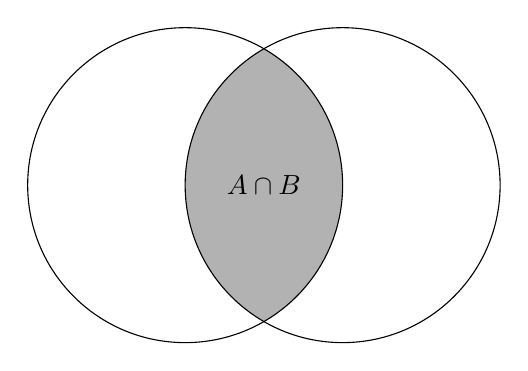
\begin{tikzpicture}
			\path[save path=\pathA](-1,0)circle(2cm);
			\path[save path=\pathB](1,0)circle(2cm);
			\begin{scope}
				\clip[use path=\pathA];
				\fill[black!30][use path=\pathB];
			\end{scope}
			\draw[use path=\pathA];
			\draw[use path=\pathB];
			\draw(0,0)node{\(A \cap B\)};
		\end{tikzpicture}
		\subcaption{集合的交}
	\end{subfigure}%
	\begin{subfigure}[b]{\subwidth}
		\centering
		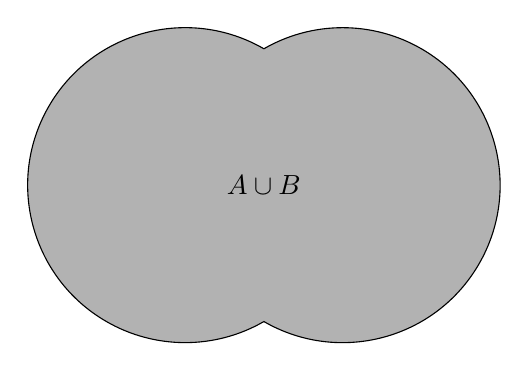
\begin{tikzpicture}
			\filldraw[fill=black!30,draw=black]
				(0,{sqrt(3)})arc[start angle=60,end angle=300,radius=2]
				arc[start angle=240,end angle=480,radius=2];
			\draw(0,0)node{\(A \cup B\)};
			\pgfresetboundingbox
			\path[use as bounding box] (-3,-2)rectangle(3,2);
		\end{tikzpicture}
		\subcaption{集合的并}
	\end{subfigure}%

	\begin{subfigure}[b]{\linewidth}
		\centering
		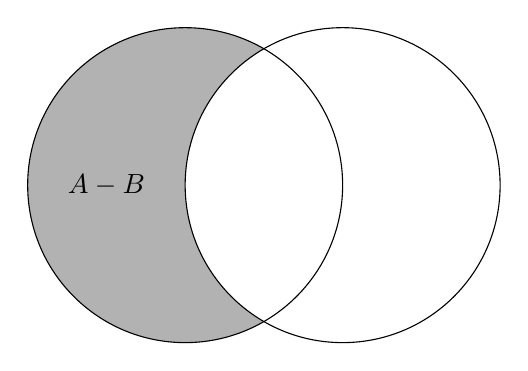
\begin{tikzpicture}
			\fill[black!30](0,{sqrt(3)})arc[start angle=60,end angle=300,radius=2]
				arc[start angle=240,end angle=120,radius=2];
			\draw(-1,0)circle(2cm);
			\draw(1,0)circle(2cm);
			\draw(-2,0)node{\(A-B\)};
			\pgfresetboundingbox
			\path[use as bounding box] (-3,-2)rectangle(3,2);
		\end{tikzpicture}
		\subcaption{集合的差}
	\end{subfigure}%
	\caption{韦恩图}
	\label{figure:集合论.韦恩图}
\end{figure}

\begin{property}
集合的运算满足以下性质:
\begin{enumerate}
\item 幂等律
\begin{gather}
	A \cap A = A, \\
	A \cup A = A.
\end{gather}

\item 交换律({\rm Commutative laws})
\begin{gather}
	A \cap B = B \cap A, \label{equation:集合论.集合代数公式1-1} \\
	A \cup B = B \cup A. \label{equation:集合论.集合代数公式1-2}
\end{gather}

\item 结合律({\rm Associative laws})
\begin{gather}
	(A \cap B) \cap C = A \cap (B \cap C), \label{equation:集合论.集合代数公式2-1} \\
	(A \cup B) \cup C = A \cup (B \cup C). \label{equation:集合论.集合代数公式2-2}
\end{gather}

\item 分配律({\rm Distributive laws})
\begin{gather}
	(A \cap B) \cup C = (A \cup C) \cap (B \cup C), \label{equation:集合论.集合代数公式3-1} \\
	(A \cup B) \cap C = (A \cap C) \cup (B \cap C), \label{equation:集合论.集合代数公式3-2} \\
	A \cup \bigcap \mathscr{B} = \bigcap\Set{A \cup X \given X \in \mathscr{B}}, \quad(\mathscr{B}\neq\emptyset) \label{equation:集合论.集合代数公式3-3} \\
	A \cap \bigcup \mathscr{B} = \bigcup\Set{A \cap X \given X \in \mathscr{B}}, \label{equation:集合论.集合代数公式3-4} \\
	\Powerset (A \cup B) \supseteq \Powerset A \cup \Powerset B, \label{equation:集合论.集合代数公式3-5} \\ %@see: 《Elements of Set Theory》 P26 Exercise 7(b).
	\Powerset (A \cap B) = \Powerset A \cap \Powerset B. \label{equation:集合论.集合代数公式3-6} %@see: 《Elements of Set Theory》 P26 Exercise 7(a)
\end{gather}

%@see: https://mathworld.wolfram.com/deMorgansLaws.html
\item 对偶律({\rm De Morgan's laws})(假设\(\mathscr{A}\neq\emptyset\))
\begin{gather}
	\Omega - (A \cap B)
	= (\Omega - A) \cup (\Omega - B), \label{equation:集合论.集合代数公式4-1} \\
	\Omega - (A \cup B)
	= (\Omega - A) \cap (\Omega - B), \label{equation:集合论.集合代数公式4-2} \\
	\Omega - \bigcup\mathscr{A}
	= \bigcap\Set{\Omega - X \given X\in\mathscr{A}}, \label{equation:集合论.集合代数公式4-3} \\
	\Omega - \bigcap\mathscr{A}
	= \bigcup\Set{\Omega - X \given X\in\mathscr{A}}. \label{equation:集合论.集合代数公式4-4}
\end{gather}

\item 与空集\(\emptyset\)和全集\(\Omega\)的运算(假设\(A \subseteq \Omega\))
\begin{gather}
	A \cup \emptyset = A, \label{equation:集合论.集合代数公式5-1} \\
	A \cap \emptyset = \emptyset, \label{equation:集合论.集合代数公式5-2} \\
	A \cup \Omega = \Omega, \label{equation:集合论.集合代数公式5-3} \\
	A \cap \Omega = A, \label{equation:集合论.集合代数公式5-4} \\
	A \cup (\Omega - A) = \Omega, \label{equation:集合论.集合代数公式5-5} \\
	A \cap (\Omega - A) = \emptyset, \label{equation:集合论.集合代数公式5-6} \\
	A \cup (A \cap B) = A, \\
	A \cap (A \cup B) = A, \\
	\Omega - \emptyset = \Omega, \\
	\Omega - \Omega = \emptyset, \\
	\Omega - (\Omega - A) = A.
\end{gather}

\item 包含关系
\begin{gather}
	A \subseteq B \implies A \cup C \subseteq B \cup C, \label{equation:集合论.集合代数公式6-1} \\
	A \subseteq B \implies A \cap C \subseteq B \cap C, \label{equation:集合论.集合代数公式6-2} \\
	A \subseteq B \implies \bigcup A \subseteq \bigcup B, \label{equation:集合论.集合代数公式6-3} \\
	A \subseteq B \implies (\Omega - B) \subseteq (\Omega - A), \label{equation:集合论.集合代数公式6-4} \\
	\emptyset \neq A \subseteq B \implies \bigcap B \subseteq \bigcap A, \label{equation:集合论.集合代数公式6-5} \\
	A \cap B \subseteq A, \\
	A \subseteq A \cup B.
\end{gather}

\item 差集
\begin{gather}
	A - B \subseteq A, \\
	B \subseteq \Omega
	\implies
	A - B = A \cap (\Omega - B), \\
	A \cup B = B
		\iff A \subseteq B
		\iff A \cap B = A
		\iff A - B = \emptyset, \label{equation:集合论.集合代数公式7-3} \\
	A \symdiff B = B \symdiff A, \\
	(A \symdiff B) \symdiff C = A \symdiff (B \symdiff C), \\
	A \symdiff \emptyset = A, \\
	A \symdiff A = \emptyset, \\
	A \symdiff B = A \symdiff C
		\iff B = C.
\end{gather}
\end{enumerate}
\begin{proof}
对\cref{equation:集合论.集合代数公式1-1} 证明如下:
\begin{align*}
	x \in A \cap B
	&\iff x \in A \land x \in B \\
	&\iff x \in B \land x \in A \\
	&\iff x \in B \cap A.
\end{align*}

对\cref{equation:集合论.集合代数公式1-2} 证明如下:
\begin{align*}
	x \in A \cup B
	&\iff x \in A \lor x \in B \\
	&\iff x \in B \lor x \in A \\
	&\iff x \in B \cup A.
\end{align*}

对\cref{equation:集合论.集合代数公式2-1} 证明如下:
\begin{align*}
	x \in (A \cap B) \cap C
	&\iff x \in A \cap B \land x \in C \\
	&\iff (x \in A \land x \in B) \land x \in C \\
	&\iff x \in A \land (x \in B \land x \in C) \\
	&\iff x \in A \land x \in B \cap C \\
	&\iff x \in A \cap (B \cap C).
\end{align*}

对\cref{equation:集合论.集合代数公式2-2} 证明如下:
\begin{align*}
	x \in (A \cup B) \cup C
	&\iff x \in A \cup B \lor x \in C \\
	&\iff (x \in A \lor x \in B) \lor x \in C \\
	&\iff x \in A \lor (x \in B \lor x \in C) \\
	&\iff x \in A \lor x \in B \cup C \\
	&\iff x \in A \cup (B \cup C).
\end{align*}

对\cref{equation:集合论.集合代数公式3-5} 证明如下:
\begin{align*}
	x \in \Powerset A \cup \Powerset B
	&\iff x \in \Powerset A \lor x \in \Powerset B \\
	&\iff x \subseteq A \lor x \subseteq B \\
	&\implies x \subseteq A \cup B \\
	&\iff x \in \Powerset (A \cup B),
\end{align*}
注意到中间步骤的\(\implies\)通常不是可逆的,
这是因为只要取\(a \subseteq A - B, b \subseteq B - A, x = a \cup b\),
就有\(x \subseteq A \cup B\)但是\(x \not\subseteq A \land x \not\subseteq B\),
因此\(x \subseteq A \cup B \notimplies x \subseteq A \lor x \subseteq B\).
%从上面的证明过程可以看出,
%要使\(\Powerset (A \cup B) = \Powerset A \cup \Powerset B\)成立,
%必有\[
%	\forall x \bigl(
%		x \subseteq A \cup B
%		\iff
%		x \subseteq A \lor x \subseteq B
%	\bigr)
%\]成立.
%取\(x = A \cup B\),
%由\(x \subseteq A \lor x \subseteq B\)
%可得\[
%	A \cup B = A \lor A \cup B = B.
%\]
%因此,当且仅当\(A \cup B \in \Set{A,B}\)时,
%就有\(\Powerset (A \cup B) = \Powerset A \cup \Powerset B\)成立.

对\cref{equation:集合论.集合代数公式3-6} 证明如下:
\begin{align*}
	x \in \Powerset (A \cap B)
	&\iff x \subseteq A \cap B \\
	&\iff x \subseteq A \land x \subseteq B \\
	&\iff x \in \Powerset A \land x \in \Powerset B \\
	&\iff x \in \Powerset A \cap \Powerset B.
\end{align*}

对\cref{equation:集合论.集合代数公式6-5} 证明如下:
\begin{align*}
	A \subseteq B
	&\iff (\forall t)[t \in A \implies t \in B] \\
	&\implies (\forall x)[
		(\forall b)[b \in B \implies x \in b]
		\implies
		(\forall a)[a \in A \implies x \in a]
	] \\
	&\iff (\forall x)[x \in \bigcap B \implies x \in \bigcap A].
	\qedhere
\end{align*}
\end{proof}
\end{property}

\begin{example}
%@see: 《Elements of Set Theory》 P32 Exercise 21.
设\(A,B\)是集合.
证明:\begin{equation}\label{equation:集合论.并集的并等于并的并集}
	\bigcup(A \cup B) = \bigcup A \cup \bigcup B.
\end{equation}
\begin{proof}
直接计算得
\begin{align*}
	x \in \bigcup(A \cup B)
	&\iff
	(\exists t)[t \in A \cup B \implies x \in t] \\
	&\iff
	(\exists t)[t \in A \lor t \in B \implies x \in t] \\
	&\iff
	(\exists t)[t \in A \implies x \in t] \lor (\exists t)[t \in B \implies x \in t] \\
	&\iff
	x \in \bigcup A \lor x \in \bigcup B \\
	&\iff
	x \in \bigcup A \cup \bigcup B.
	\qedhere
\end{align*}
\end{proof}
\end{example}

\begin{example}
%@see: 《Elements of Set Theory》 P32 Exercise 22.
设\(A,B\)是非空集合.
证明:\begin{equation}
	\bigcap(A \cup B) = \bigcap A \cap \bigcap B.
\end{equation}
%\begin{proof}
%直接计算得
%\begin{align*}
%	x \in \bigcap(A \cup B)
%	&\iff
%	x \in \bigcap A \land x \in \bigcap B \\
%	&\iff
%	x \in \bigcap A \cap \bigcap B.
%	\qedhere
%\end{align*}
%\end{proof}
\end{example}

\begin{example}
证明:\begin{equation}
	(A \cup B) - (A \cap B) = (A-B)\cup(B-A).
\end{equation}
\begin{proof}
根据集合交、并、差的定义,有
\begin{align*}
	x \in (A \cup B) - (A \cap B)
	&\iff x \in (A \cup B) \land x \notin (A \cap B) \\
	&\iff (x \in A \lor x \in B) \land \neg(x \in A \land x \in B) \\
	&\iff (x \in A \land \neg(x \in A \land x \in B))
	 \lor (x \in B \land \neg(x \in A \land x \in B)) \\
	&\iff (x \in A \land (x \notin A \lor x \notin B))
	 \lor (x \in B \land (x \notin A \lor x \notin B)) \\
	&\iff (x \in A \land x \notin B) \lor (x \in B \land x \notin A) \\
	&\iff x \in (A-B)\cup(B-A).
\qedhere
\end{align*}
\end{proof}
\end{example}
